\documentclass[11pt,a4paper]{report}
\usepackage[utf8]{inputenc}
\usepackage{amsmath}
\usepackage{amsfonts}
\usepackage{amssymb}
\usepackage{graphicx}
\usepackage{enumitem}
\usepackage[left=2cm, right=2cm, top=4.5cm, bottom=2cm]{geometry}

\begin{document}
	%Portada
	\begin{titlepage}
		\centering
		{\scshape\LARGE Universidad Nacional Autónoma de México \par}
		\vspace{1cm}
		{\scshape\Large Probabilidad I\par}
		\vspace{1.5cm}
		{\huge\bfseries Tarea VI\par}
		\vspace{.5cm}

		{\Large\itshape Alan Ernesto Arteaga Vázquez \par}
		 \vspace{.5cm}
		{\Large\itshape Raúl Llamosas Alvarado \par}
		 \vspace{.5cm}
		{\Large\itshape Edgar Quiroz Castañeda \par}
	    \vspace{.5cm}
		{\Large\itshape Jean Paul Ruiz Melo\par}
		\vspace{.5cm}
		{\Large\itshape Sandra Del Mar Soto Corderi \par}

		\vfill
		 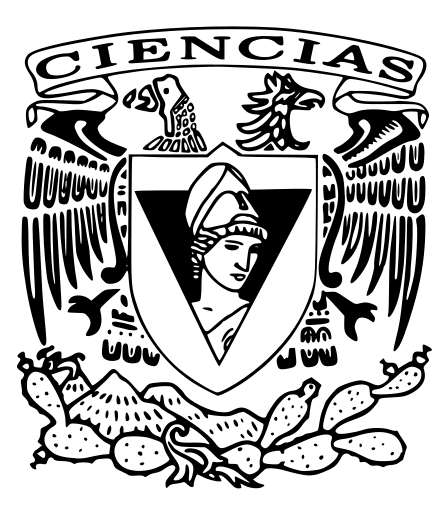
\includegraphics[width=0.3\textwidth]{escudo.png}
		\vfill

		{\large Martes 20 de noviembre del 2018 \par}
	\end{titlepage}

	\pagebreak
	\setlength{\voffset}{-0.75in}
	\setlength{\headsep}{5pt}

	%Ejericios
	\begin{enumerate}
		%1
		\item{
			Sea $X\sim\text{Poisson}(\lambda)$, demuestre que
            \[F_X(n) = \frac{1}{n!}\int_{\lambda}^{\infty}e^{-x}x^n dx\]
			Resolviendo la integral por partes, tenemos que
			\[\int_{\lambda}^{\infty}e^{-x}x^n dx
			= -e^{-x}x^n \Big|_{\lambda}^{\infty}+
			n\int_{\lambda}^{\infty}{e^{-x}x^{n-1}dx}
			= e^{-\lambda}\lambda^n + n\int_{\lambda}^{\infty}{e^{-x}x^{n-1}dx}\]
			Repitiendo este proceso $n$ veces, tenemos que la integral es de la
			forma
			\begin{align*}
				\int_{\lambda}^{\infty}e^{-x}x^n dx
				&= e^{-\lambda}\lambda^n + n(e^{-\lambda}\lambda^{n-1} +
				(n-1)(e^{-\lambda}\lambda^{n-2} + \dots + 2(e^{-\lambda}\lambda +
				e^{-\lambda})\dots))\\
				&= e^{-\lambda}\lambda^n + ne^{-\lambda}\lambda^{n-1} +
				n(n-1)e^{-\lambda}\lambda^{n-2} + \dots
				+ n(n-1)\dots(2)e^{-\lambda}\lambda + n!e^{-\lambda}
			\end{align*}
			Entonces
			\begin{align*}
				\frac{1}{n!}\int_{\lambda}^{\infty}e^{-x}x^n dx
				&= \frac{1}{n!}(e^{-\lambda}\lambda^n + ne^{-\lambda}\lambda^{n-1} +
				n(n-1)e^{-\lambda}\lambda^{n-2} + \dots n!e^{-\lambda} )\\
				&= \frac{e^{-\lambda}\lambda^n}{n!} + \frac{ne^{-\lambda}\lambda^{n-1}}{n!}
				+ \frac{n(n-1)e^{-\lambda}\lambda^{n-2}}{n!} + \dots +
				\frac{n!e^{-\lambda}}{n!}\\
				&= \frac{e^{-\lambda}\lambda^n}{n!} +
				\frac{e^{-\lambda}\lambda^{n-1}}{(n-1)!} +
				\frac{e^{-\lambda}\lambda^{n-2}}{(n-2)!} + \dots +
				e^{-\lambda}\lambda + e^{-\lambda}
			\end{align*}
			Por otra parte, como $X\sim\text{Poisson}(\lambda)$, entonces
			su densidad es
			\[f_X(n) = \frac{e^{-\lambda}\lambda^{n}}{n!}\]
			con $x = \{0, 1, 2, 3, ...\}$.\\
			Luego, por definición de distribución,
			\[F_X(n) = \sum_{i=0}^{n}{\frac{e^{-\lambda}\lambda^{i}}{i!}}
			= e^{-\lambda} + e^{-\lambda}\lambda^{1} + \frac{e^{-\lambda}\lambda^{2}}{2}
			+ \dots  + \frac{e^{-\lambda}\lambda^{n-1}}{(n-1)!} +
			\frac{e^{-\lambda}\lambda^n}{n!}\]
			Que es exactamente la expansión de la integral. Por lo tanto,
			\[F_X(n) = \frac{1}{n!}\int_{\lambda}^{\infty}e^{-x}x^n dx\]
		}

		%2
		\item{
			Suponga que en un grupo de probabilidad de 100 alumnos, el 85\% de
            los alumnos reprobó el segundo examen parcial. Si tomamos una
            muestra de tamaño 30. Calcule la probabilidad de
            \begin{enumerate}
                %a
                \item {
                	Exactamente 10 alumnos de la muestra hayan reprobado.\\
					Esto implicaría que 20 alumnos de la muestra aprobaron,
					lo cuál es imposible pues sólo 15 aprobaron.
					Entonces la probabilidad de que eso pase es 0.
                }

                %b
                \item {
                	Al menos 5 alumnos de la muestra hayan reprobado.\\
					Como sólo 15 aprobaron, entonces al menos 15 reprobaron.
					En particular, siempre se tiene que al menos 5 aprobaron.
					Entonces eso probabilidad es 1.
                }

                %c
                \item {
                	El número de alumnos reprobados de la muestra esté entre 5 y 10.\\
					Hay al menos 15 alumnos reprobados. Entonces, nunca hay entre
					5 y 20 reprobados. Entonces, la probabilidad de eso es 0.
                }
            \end{enumerate}
		}

		%3
		\item{
            Una aseguradora tiene 10 pólizas independientes con una cobertura
            de una año. El valor nominal de cada una de esas pólizas es de
            \$1,000. La probabilidad de que haya una reclamación en el año en
            consideración es de 0.1. Encuentre la probabilidad de que la
            aseguradora pague más del total esperado para el año en
            consideración.\\
			Sea $X$ la variable aleatoria que representa el número de polizas
			a pagar en el año. Tenemos que cada póliza es independiente de las
			demás, y cada una tiene probabilidad de 0.1 de ser pagada.\\
			Entonces, si consideramos que el pagar una poliza es un éxito,
			tenemos que $X \sim  Bin(0.1, 10)$, por lo que
			\[f_X(x) = {10 \choose x}(0.1)^x (0.9)^{10-x}\]
			Y la esperanza, o sea el número esperado de pólizas a pagar, es
			\[E(X) = np = 10 \times 0.1 = 1\]
			Por lo que se espera pagar una póliza, es decir \$1000.\\
			Entonces se busca
			\[P(X > 1) = 1 - P(X \leq 1) = 1 - P(X = 0) - P(X = 1) = 1 - f_X(0) - f_X(1)\]
			Tenemos que
			\begin{align*}
				&f_X(0) = {10 \choose 0}(0.1)^0 (0.9)^{10} = (0.9)^{10} \approx 0.35 \\
				&f_X(1) = {10 \choose 1}(0.1)^1 (0.9)^9 = 0.1 \cdot (0.9)^9 \approx 0.04\\
				&\implies P(X > 1) = 1 - (0.9)^{10} - 0.1 \cdot (0.9)^9 \approx 0.61
			\end{align*}
			Entonces, hay una probabilidad de más o menos $61\%$ de que la
			aseguradora pague más de lo esperado.
		}

		%4
		\item{
			Una moneda es lanzada tantas veces como sea necesario hasta obtener
            5 águilas. Si se sabe que en los primeros 8 lanzamientos no se ha
            logrado el objetivo. Calcule la probabilidad de que se requieran, en
            total, menos de 12 lanzamientos.\\
			Se busca la probabilidad de que se logre obtener las 5 águilas en 9,
			10 u 11 lanzamientos, dado que no se han obtenido las 5 águilas en
			los 8 primero lanzamientos. Es decir, la probabilidad de obtener a
			los más 6 fracasos antes del quinto éxito dado que han ocurrido
			al menos 4 fracasos. \\
			Esto es una distribución binomial negativa.\\
			Es decir $X \sim BinNeg(\frac{1}{2}, 5)$. Esto significa que
			\[f_X(x) = {x+5-1 \choose x} \frac{1}{2}^5 \frac{1}{2}^x =
			{x+5-1 \choose x} \frac{1}{2}^{5+x}\]
			Como estas probabilidades son independientes entonces la probabilidad
			de que ocurra alguna de ellas es la suma de las probabilidades.
			\[f_X(0) = {4 \choose 0} \frac{1}{2}^{5} = \frac{1}{32}\]
			\[f_X(1) = {5 \choose 1} \frac{1}{2}^{6} = \frac{5}{64}\]
			\[f_X(2) = {6 \choose 2} \frac{1}{2}^{7} = \frac{15}{128}\]
			\[f_X(3) = {7 \choose 3} \frac{1}{2}^{8} = \frac{35}{256}\]
			\[f_X(4) = {8 \choose 4} \frac{1}{2}^{9} = \frac{70}{512}\]
			\[f_X(5) = {9 \choose 5} \frac{1}{2}^{10} = \frac{126}{1024}\]
			\[f_X(6) = {10 \choose 6} \frac{1}{2}^{11} = \frac{210}{2048}\]
			\begin{align*}
				P(X \leq 6 | X \geq 4) &= \frac{P(X \leq 6 \cap X \geq 4)}{P(X \geq 4)}\\
							  &=\frac{P(X \leq 6 \cap X \geq 4)}{1-P(X < 4)}  \\
							  &=\frac{f_X(4) + f_X(5) + f_X(6)}
							  {1-(f_X(0) + f_X(1) + f_X(2)+ f_X(3))}  \\
							  &= \frac{\frac{140+126+105}{1024}}
							  {1-\frac{8+20+30+35}{256}} \\
							  &= \frac{\frac{371}{1024}}{1-\frac{93}{256}} \\
							  &= \frac{\frac{371}{1024}}{\frac{163}{256}} \\
							  &= \frac{371}{652} \\
							  &\approx 0.57
			\end{align*}
		}

		%5
		\item{
			Un dado balanceado es lanzado hasta que cae la cara con el "4". Si X
            es el número de lanzamientos requeridos hasta obtener el primer "4".
            ¿Cuál es el valor de $\epsilon$ más pequeño para el cual
            $P(X \leq \epsilon) \geq 0.5$?
		}

		%6
		\item{
			En una tienda de abarrotes se venden 400 artículos, 6 de los cuales
            no tienen marcada la clave de su precio. Si una persona entra a la
            tienda y elige 10 artículos, calcule la probabilidad de que entre
            los  artículos escogidos haya por lo menos un artículo que no tenga
            marcada la cave de su precio.
		}

		%7
		\item{
			Supongamos que el 5\% de las personas mayores de 18 años tiene su
            INE vencida. Utilice la aproximación Poisson para estimar la
            probabilidad de que a lo más 3 de 50 personas mayores de 18 años,
            seleccionadas al azar, tengan su INE vencida.
		}

		%8
		\item{
			\begin{enumerate}
				%a
				\item {
					Encuentre la moda de la distribución gamma.
				}

				%b
				\item {
					Si $X \sim \text{exp}(\lambda)$, demuestre que
                        $$ \mathbb{E}(X^k) = \frac{k!}{\lambda^k} $$
				}

			\end{enumerate}
		}

		%9
		\item{
			Sea X una variable aleatoria continua con función de distribución F.
            Defínase Y una variable aleatoria tal que $Y = F(X)$. Demuestre que
            $Y \sim \text{Unif}(0,1)$.
		}

		%10
		\item{
			Conteste las siguientes preguntas respecto a la distribución normal.
			\begin{enumerate}
				%a
				\item {
					Demuestre que la función de densidad $N(\mu, \sigma^2)$ es
                    simétrica con respecto a $x = \mu$, alcanza su máximo en
                    $x = \mu$ y tiene puntos de inflexión en $x_1= \mu + \sigma$
                    y $x_2 = \mu - \sigma$.
				}

				%b
				\item {
					Si X es una variable aleatoria con distribución normal con
                    parámetros $\mu = 10$ y $\sigma^2 = 36$.\\
                    Calcule: $\mathbb{P}(X > 5)$, $\mathbb{P}(4 < X < 10)$,
                    $\mathbb{P}(X < 8)$, $\mathbb{P}(X < 20)$ y
                    $\mathbb{P}(X > 16)$.
				}

				%c
				\item {
					Suponga que $X$ es una variable aleatoria con media y
					varianza igual a 20- ¿Qué se puede decir de
					$\mathbb{P}(0 \leq X \leq 40)$?
				}

				%d
				\item {
					Sea $X$ una variable aleatoria con distribución normal con
					media 12 y varianza 4. Encontrar el valor de $\tau$ tal que
					$\mathbb{P}(X < \tau) \in \{0,1\}$.
				}

				%e
				\item {
					Si $X$ tiene una distribución normal con media $\mu = 9$ y
					varianza $\sigma^2 = 4$, encontrar \\
					$\mathbb{P}(X^2 - 2X \leq 8)$
				}
			\end{enumerate}
		}

		%11
		\item{
			Sea $X$ una variable aleatoria con distribución uniforme en el
			intervalo $(-\frac{\pi}{2}, \frac{\pi}{2})$. Encuentre la función de
			distribución y la función de densidad $Y = \tan(X)$.
		}

		%12
		\item{
			Si $X \sim \text{Unif}(0, 10)$, calcular
			$\mathbb{P}(X + \frac{10}{X} > 7)$
		}

		%13
		\item{
			Un aparato mide y graba de manera continua la actividad sísmica de
			una región remota. El tiempo, $T$, de falla del aparato se
			distribuye exponencial con media de 3 años. Debido a que el aparato
			no será monitoreado durante sus dos primeros años de servicio, el
			tiempo para descubrir una falla es $X = \text{máx}\{T,2\}$.
			Encuentre $\mathbb{E}(X)$.
		}

		%14
		\item{
			Demuestre que si $X \sim \text{Hipergeométrica}(N,m,n)$, entonces.
				$$ \sum_{x = 0}^{n}f_X(x) = 1$$
		}

		%15
		\item{
			Sea $X$ una variable aleatoria con distribución binomial con
			parámetros n y p. Demuestre
			\begin{enumerate}
				%a
				\item {
					$\mathbb{P}(X = x + 1) = \frac{p}{1 - p} \frac{n - x}{x + 1}
					 \mathbb{P}(X = x)$
				}

				%b
				\item {
					$\mathbb{P}(X \in \{ 1,3,5,...\}) = \frac{1}{2}
					 (1 - (1 - 2p)^2)$
				}

				%c
				\item {
					$\mathbb{P}(X \in \{ 0,2,4,...\}) = \frac{1}{2}
					 (1 + (1 - 2p)^2)$
				}
			\end{enumerate}
		}

		%16
		\item{
		Sea $X$ una variable aleatoria con distribución Poisson con parámetro
		$\lambda$. Demuestre
			\begin{enumerate}
				%a
				\item {
					$\mathbb{P}(X = x + 1) = \frac{\lambda}{x + 1}
					 \mathbb{P}(X = x)$
				}

				%b
				\item {
					$\mathbb{P}(X \in \{ 1,3,5,...\}) = \frac{1}{2}
					 (1 - e^{-2\lambda})$
				}

				%c
				\item {
					$\mathbb{P}(X \in \{ 0,2,4,...\}) = \frac{1}{2}
					 (1 + e^{-2\lambda})$
				}
			\end{enumerate}
		}

		%17
		\item{
			Si $X \sim \text{Poisson}(\lambda)$, y además $\mathbb{P}(X \leq 1)
			= 2\mathbb{P}(X = 2)$
		}

		%18
		\item{
			Si $X$ es una variable aleatoria con distribución Poisson tal que
			$\mathbb{P}(X = 0) = \mathbb{P}(X = 1)$, encuentre $\mathbb{E}(X)$.
		}

		%19
		\item{
			Un componente con tiempo de vida que se distribuye exponencialmente
			con una tasa de falla de 1 por 24 horas se pone en servicio con un
			componente de reemplazo del mismo tipo que se sustituye por el
			primero cuando falla. ¿Cuál es la mediana del tiempo total hasta la
			falla de ambos componentes?
		}

		%20
		\item{
			Sea $U$ una variable aleatoria con distribución uniforme continua
			con parámetros 0,1. Se define a $X = a+(b - a)U$.Encuentre
			\begin{enumerate}
				%a
				\item {
					$\mathbb{E}(X)$
				}

				%b
				\item {
					$\text{Var}(X)$
				}
			\end{enumerate}

		}

	\end{enumerate}
\end{document}
